\documentclass[10pt]{beamer}

\usepackage[ngerman]{babel}
\usepackage{amsmath}
\usepackage{bbm}
\usepackage{tikz}

\usepackage{tabularx}
\usepackage{graphicx}
\usepackage{subfig}
\usepackage{url}
%\usepackage{hyperref}
\usepackage{eurosym}
\usepackage{listings}
\usepackage{datetime}
\usepackage[style=authoryear, backend=biber]{biblatex}

\usepackage{epstopdf}

\usepackage{multirow}
\usepackage{colortbl}
\usepackage{booktabs}
%\usepackage{setspace}

\newif\ifzihbackground
\zihbackgroundtrue
%\zihbackgroundfalse

% Yes, this is dirty
\newcommand\zihmaketitle{
	\definecolor{white}{gray}{1.00}%
	\setbeamercolor{normaltext}{bg=darkblue}%
	\setbeamertemplate{headline}{%
		\vskip6.15mm\color{white}\setlength{\arrayrulewidth}{0.3pt}%
		\begin{tabular*}{\paperwidth}[b]{l@{\extracolsep\fill}}%
			\hspace*{3.0mm}\color{white}%
			
\includegraphics[height=7.81mm]{theme/logo/tu_logo_black}\\[1.2mm]%
			\hline\hspace*{11.76mm}\rule[-0.8mm]{0pt}{2.47mm}%
			\def\@@dummyComma{}\rule{0pt}{5.8pt}%
			\insertinstitute \\%
			\hline%
		\end{tabular*}%
		\hspace{-\paperwidth}%
	}%
    \ifzihbackground
      \setbeamertemplate{footline}{}
      \setbeamertemplate{background}{
\includegraphics[height=\paperheight,width=\paperwidth]{theme/logo/bg}}
      \else
      \setbeamertemplate{footline}{
          \parbox[t][22mm]{\paperwidth}{
              \vspace*{-8.18mm}
              \rule
              {98.6mm}{0pt}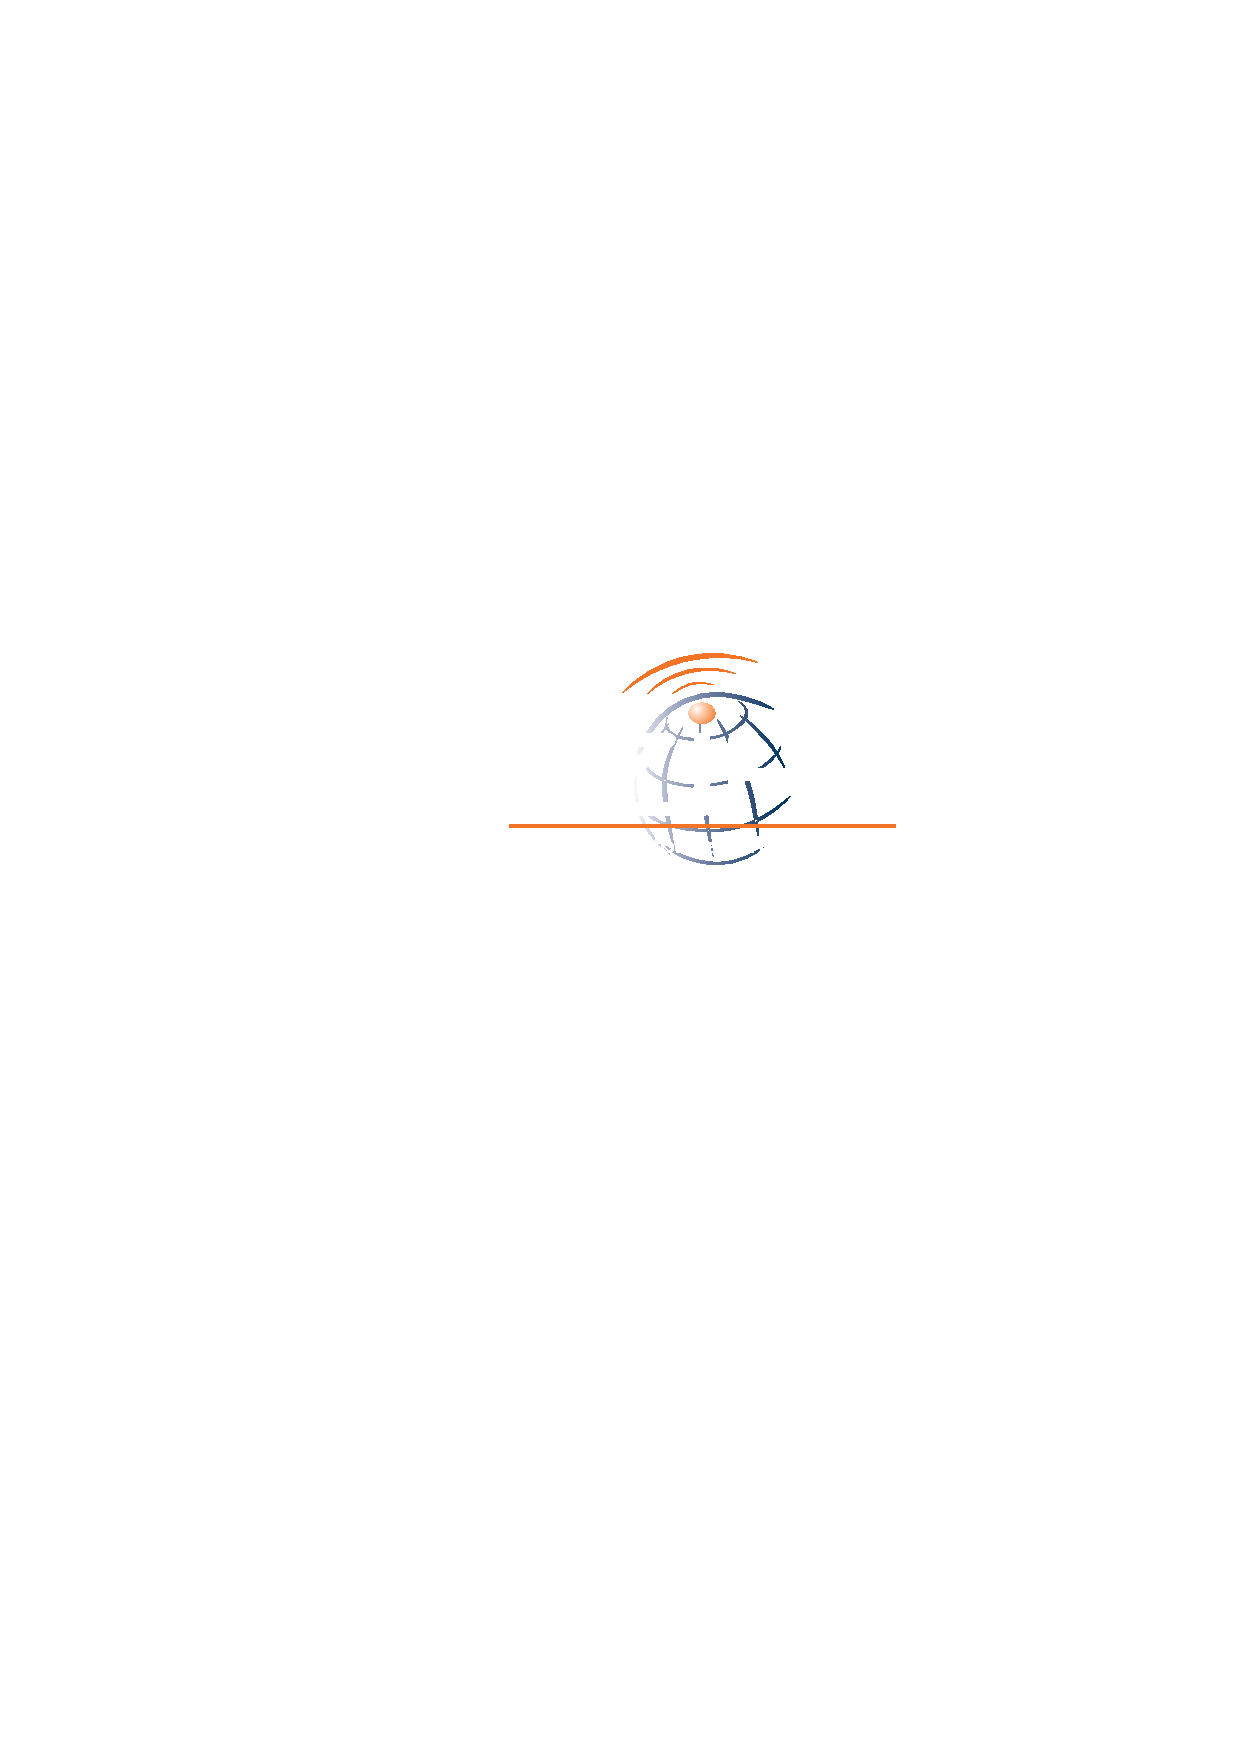
\includegraphics[height=15mm]{theme/logo/zih_logo_white}

          }
      }
    \fi%
   \frame{\titlepage}
    % Kopf-/Fusszeilen fuer restliche Folien
    \setbeamercolor{normal text}{bg=white}
    \setbeamertemplate{background}{}
    \setbeamertemplate{headline}[zih01 theme]
    \setbeamertemplate{footline}[zih01 theme]
}

\usetheme{Dresden}
%\useoutertheme{theme/zih01}
%\useinnertheme{theme/zih01}
\usepackage{theme/beamerouterthemezih01}
\usepackage{theme/beamerinnerthemezih01}

%\useinnertheme{rounded}
\definecolor{darkblue}{rgb}{0.04, 0.16, 0.32}
% font color for headlines etc.
\setbeamercolor*{structure}{fg=darkblue,bg=white}
% disable navigation symbols
\setbeamertemplate{navigation symbols}{}
% can't remember what this is good for
\setbeamercovered{transparent}

% reduce margin size
\setbeamersize{text margin left=0.7cm}
\setbeamersize{text margin right=0.7cm}
%
% Outer Color Theme "whale" sorgt f?r strenge farbliche Trennen zwischen Zierrat
% und dem eigentlichen Inhalt. Ein dunkler Hintergrund f?r den Folientitel wirkt
% aber zu aufdringlich.
%
\usecolortheme{orchid}
%\setbeamercolor{titlelike}{parent=structure}

%
% Inner Color Theme "orchid" sorgt f?r farblich abgesetzt Bl?cke (Definitionen,
% S?tze, Beispiele, Beweise, ...).
%
%\usecolortheme{orchid}

%zum drucken
%\usepackage{pgfpages}
%\pgfpagesuselayout{resize to}[a4paper,border shrink=5mm,port]
%\pgfpagesuselayout{4 on 1}[a4paper,border shrink=3mm, landscape]

%%%%%%%%%%%%%%%%%%%%%%%%%%%%

\definecolor{LightGray}		{gray}{0.9}
\definecolor{Gray}		{gray}{0.5}
\definecolor{DarkGray}     	{gray}{0.2}
\definecolor{listinggray} 	{gray}{0.96}
\definecolor{DarkGreen}     	{rgb}{0.0,0.6,0.0}
\definecolor{DarkRed}     	{rgb}{0.6,0.0,0.0}
\definecolor{DarkBlue}     	{rgb}{0.0,0.0,0.6}
\definecolor{DarkCyan}     	{rgb}{0.7,0.7,0.2}
\definecolor{DarkDarkGreen}	{rgb}{0.0,0.4,0.0}

\lstset{language=C}
\lstset{linewidth=0.99\textwidth}
%\lstset{boxpos=c}
\lstset{xleftmargin=0.03\textwidth}
%\lstset{breaklines=true}
\lstset{framexleftmargin=0.03\textwidth}
\lstset{abovecaptionskip=\smallskipamount}
\lstset{belowcaptionskip=\smallskipamount}
\lstset{basicstyle=\ttfamily\tiny}
\lstset{backgroundcolor=\color{listinggray}}
%\lstset{frameround=ffff}
%\lstset{frame=shadowbox}
%\lstset{rulesepcolor=\color{Gray}}
\lstset{numbers=left}
\lstset{numberstyle=\tiny \color{DarkGray}}
\lstset{numbersep=0.01\textwidth}
\lstset{showstringspaces=false}
%\lstset{showspaces=false}
\lstset{tabsize=4}

%% all words in the following list are printed in bold letters in a listing 
\lstset{emph={__asm__, __volatile__, return, main,},emphstyle={\bfseries\color{DarkGray}}}
\lstset{captionpos=b}

% Style für C Sourcecode
\lstdefinestyle{CA}{
        language=C,
        basicstyle=\ttfamily\scriptsize,
        keywordstyle=\ttfamily\bfseries\color{DarkBlue},
        stringstyle=\ttfamily\color{DarkRed},
        commentstyle=\ttfamily\color{DarkGreen},
        identifierstyle=\ttfamily\color{DarkCyan},
        backgroundcolor=\color{listinggray},
}

%%%%%%%%%%%%%%%%%%%%%%%%%%%%

% define blocks for flowchart
\usetikzlibrary{shapes.geometric, arrows}

\tikzstyle{startstop} = [rectangle, rounded corners, minimum width=2cm, minimum height=0.5cm,text centered, draw=black, fill=red!30]
\tikzstyle{io} = [trapezium, trapezium left angle=70, trapezium right angle=110, minimum width=2cm, minimum height=0.5cm, text centered, draw=black, fill=blue!30]
\tikzstyle{process} = [rectangle, minimum width=2cm, minimum height=0.5cm, text centered, draw=black, fill=orange!30]
\tikzstyle{decision} = [diamond, minimum width=2cm, minimum height=0.5cm, text centered, draw=black, fill=green!30]
\tikzstyle{arrow} = [thick,->,>=stealth]

\newcommand{\mq}[1]{\glqq#1\grqq}

% registered, copyright und trademark zeichen
\def\TReg{\textsuperscript{\textregistered}}
\def\TCop{\textsuperscript{\textcopyright}}
\def\TTra{\textsuperscript{\texttrademark}}

\date{\today}
\institute[ZIH TUD]{Zentrum für Informationsdienste und Hochleistungsrechnen -- TU Dresden}
\title[PWFRA]{Parallelisierung des Wellenfrontrekonstruktionsalgorithmus auf Manycore-Prozessoren}
\subtitle{Zwischenpräsentation}
\author[Schenke]{Jonas~Schenke}

\DeclareCiteCommand{\citejournal}
{\usebibmacro{prenote}}
{\usebibmacro{citeindex}%
	\usebibmacro{journal}}
{\multicitedelim}
{\usebibmacro{postnote}}

\newcommand{\citeall}[1]{\citetitle{#1}, \cite{#1}, \citejournal{#1}}

%\room{}
%\address{}
%\city{}
%\phone{00}
\hsl{Prof. Dr. Wolfgang E. Nagel}
\betreuer{Dr. Michael Bussmann, Matthias Werner}
\email{jonas.schenke@tu-dresden.de}
\newdate{date}{20}{12}{2017}
\date{\displaydate{date}}

\addbibresource{referenzen.bib}

% Zu jedem Abschnitt Gliederung zeigen
\AtBeginSection[]
{
  \begin{frame}<beamer>{Gliederung}
    \tableofcontents[currentsection]
  \end{frame}
}

% auch bei subsections gliederung?
%\AtBeginSubsection[]
%{
%  \begin{frame}<beamer>{Gliederung}
%    \tableofcontents[currentsection,currentsubsection]
%  \end{frame}
%}

% bei sehr vielen sections, mehrspaltig
%\begin{frame}[shrink]
%\frametitle{Gliederung}
%\begin{multicols}{2}
%	\tableofcontents
%\end{multicols}
%\end{frame}


% alle Aufzaehlungen schrittweise zeigen
%\beamerdefaultoverlayspecification{<+->}

\setbeamercovered{transparent}

\begin{document}

\lstset{language= tcl}
\lstset{emph={words, zum, hervorheben,}}
\lstset{emphstyle={\color{blue}}}
\lstset{basicstyle=\ttfamily\bfseries\tiny}
\lstset{keywordstyle=\ttfamily\color{DarkBlue}}
\lstset{stringstyle=\ttfamily\color{DarkRed}}
\lstset{commentstyle=\ttfamily\color{DarkDarkGreen}}
\lstset{identifierstyle=\ttfamily\color{DarkCyan}}
\lstset{linewidth=0.99\textwidth}
\lstset{xleftmargin=0.03\textwidth}
\lstset{breaklines=true}
\lstset{framexleftmargin=0.03\textwidth}
\lstset{abovecaptionskip=\smallskipamount}
\lstset{belowcaptionskip=\smallskipamount}
\lstset{basicstyle=\ttfamily\tiny}
\lstset{backgroundcolor=\color{listinggray}}
\lstset{numbers=left}
\lstset{numberstyle=\tiny \color{DarkGray}}
\lstset{numbersep=0.01\textwidth}
\lstset{showstringspaces=false}
\lstset{showspaces=false}
\lstset{tabsize=4}
% Language C and Style CA defined in theme.tex

\zihmaketitle

\begin{frame}{Aufgabenstellung}
\frametitle{Aufgabenstellung}
\begin{itemize}
	\item Evaluierung des Wellenfrontrekonstruktionsalgorithmus
	\item Performance-Analyse des derzeit fast durchgängig seriellen Codes
	\item Parallelisierung der kritischen Pfade für Vielkernarchitekturen
	\item Performance-Messungen der parallelen Implementation
	\item Auswertung sowie Validierung der Ergebnisse
\end{itemize}
\end{frame}

\begin{frame}{Gliederung}
  \setcounter{tocdepth}{1} 
  \tableofcontents
  % Die Option [pausesections] koennte nuetzlich sein.
\end{frame}

\section{Evaluierung des Wellenfrontrekonstruktionsalgorithmus}

\subsection{Überblick}
\begin{frame}{Versuchsaufbau}
	\begin{tikzpicture}
		\node at (0,0) {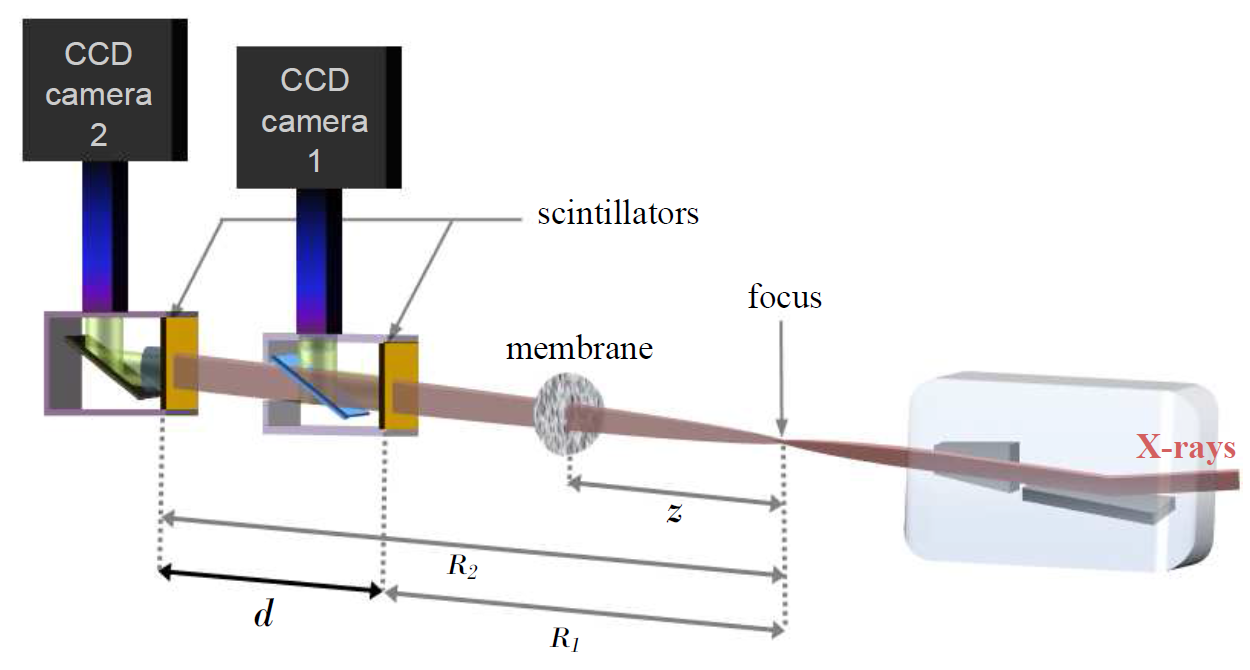
\includegraphics[width=0.98\linewidth]{./img/versuchsaufbau.png}};
		\only<2>{\draw[red, very thick] (2.4, -2.2) rectangle (5.5, -0.2);}
		\only<3>{\draw[red, very thick] (1.2, -1.2) rectangle (1.6, -0.8);}
		\only<4>{\draw[red, very thick] (-1.1, -1.4) rectangle (0.3, 0);}
		
		\only<5>{\draw[red, very thick] (-5.5, 2.9) rectangle (-1.7, -1);}
		\only<6>{\draw[red, very thick] (-4.3, -2.7) rectangle (-2.1, -2);}
		\only<7>{\draw[red, very thick] (-3.3, -1) rectangle (-1.7, 0.1);}
		
		\only<8>{\draw[red, very thick] (-3.6, 1.2) rectangle (-1.9, 2.7);}
		\only<8>{\node at (3.4,0.8) {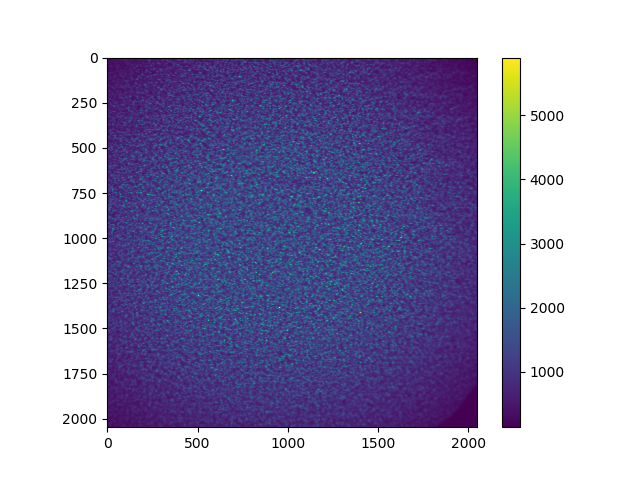
\includegraphics[width=0.5\linewidth]{img/ref_start0001_1-10}};}
		\only<8>{\draw[red, very thick] (1, 2.8) rectangle (5.8, -1.3);}
		\only<8>{\draw[red, very thick] (1, 2.8) -- (-1.9, 2.7);}
		\only<8>{\draw[red, very thick] (1, -1.3) -- (-1.9, 1.2);}
		
		\only<9>{\draw[red, very thick] (-5.3, -0.8) rectangle (-3.7, 0.3);}
		\only<10>{\draw[red, very thick] (-5.5, 1.5) rectangle (-3.8, 2.9);}
		
		\only<10>{\node at (3.4,0.8) {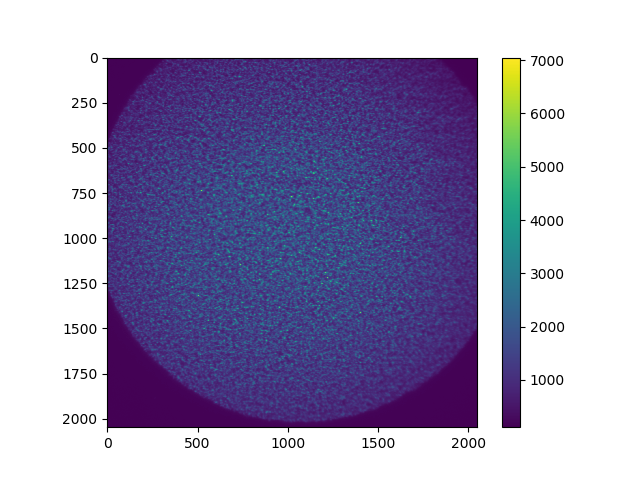
\includegraphics[width=0.5\linewidth]{img/E10001}};}
		\only<10>{\draw[red, very thick] (1, 2.8) rectangle (5.8, -1.3);}
		\only<10>{\draw[red, very thick] (1, 2.8) -- (-3.8, 2.9);}
		\only<10>{\draw[red, very thick] (1, -1.3) -- (-3.8, 1.5);}
	\end{tikzpicture}
\nocite{Ber12}
\nocite{Ber13}
\nocite{Ber15}
{\scriptsize \citeall{Ber15}}
\end{frame}

\begin{frame}{Überblick}
\textbf{Zwei Phasen:}
\begin{itemize}
	\item Initialisierungsphase
	\begin{itemize}
		\item Ermitteln des Kamerafehlers
		\item Bestimmen Ablenkung in verschiedenen Positionen \\
			$\Rightarrow$ Grundlage für Hauptroutine
	\end{itemize}
	\item<2-> Hauptroutine
	\begin{itemize}
		\item Korrigieren von Kamerafehlern ($ \rightarrow $ mit Ausgabe der Initialisierung)
		\item Ablenkung nachverfolgen
		\item Wellenfront rekonstruieren
	\end{itemize}
\end{itemize}
\end{frame}

\begin{frame}{Hauptroutine}
\only<1-5> {
	\begin{tikzpicture}
	\node at (-5,0) {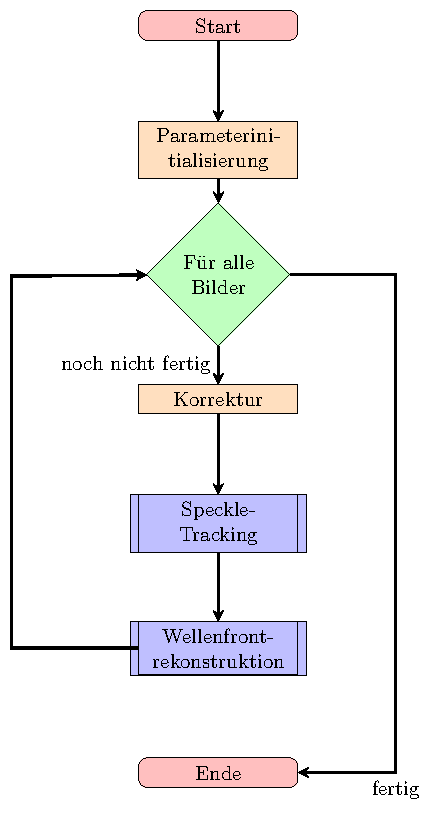
\includegraphics[width=0.35\linewidth]{tex/graph_main}};
	\only<2-4>{\node at (-2,0) {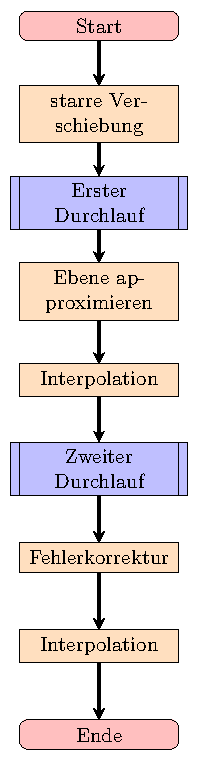
\includegraphics[width=0.17\linewidth]{tex/graph_speckle}}};
	
	\only<2>{\draw[red, very thick] (-5.9, -1.4) rectangle (-4.1, -0.7)};
	\only<2>{\draw[red, very thick] (-4.1, -0.7) -- (-3, 3.7)};
	\only<2>{\draw[red, very thick] (-4.1, -1.4) -- (-3, -3.7)};
	\only<2>{\draw[red, very thick] (-3, -3.7) rectangle (-0.9, 3.7)};
	
	
	\only<3-4>{\draw[red!25, very thick] (-5.9, -1.4) rectangle (-4.1, -0.7)};
	\only<3-4>{\draw[red!25, very thick] (-4.1, -0.7) -- (-3, 3.7)};
	\only<3-4>{\draw[red!25, very thick] (-4.1, -1.4) -- (-3, -3.7)};
	\only<3-4>{\draw[red!25, very thick] (-3, -3.7) rectangle (-0.9, 3.7)};
	
	\only<3>{\draw[red, very thick] (-2.95, 1.4) rectangle (-1.05, 2.07)};
	
	\only<4>{\draw[red, very thick] (-2.95, -1.2) rectangle (-1.05, -0.55)};
	
	\only<5>{\draw[red, very thick] (-5.9, -1.4) rectangle (-4.1, -0.7)};
	\only<5>{\node at (1,2.1) {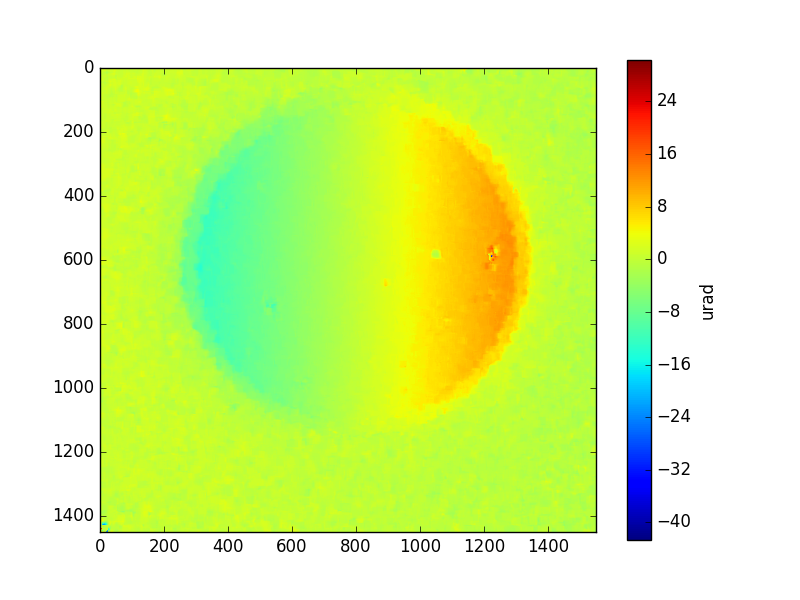
\includegraphics[width=0.4\linewidth]{img/SpeckDisH_E10001_edf_ref_start0001_1-10_edf}}};
	\only<5>{\node at (1,-1.6) {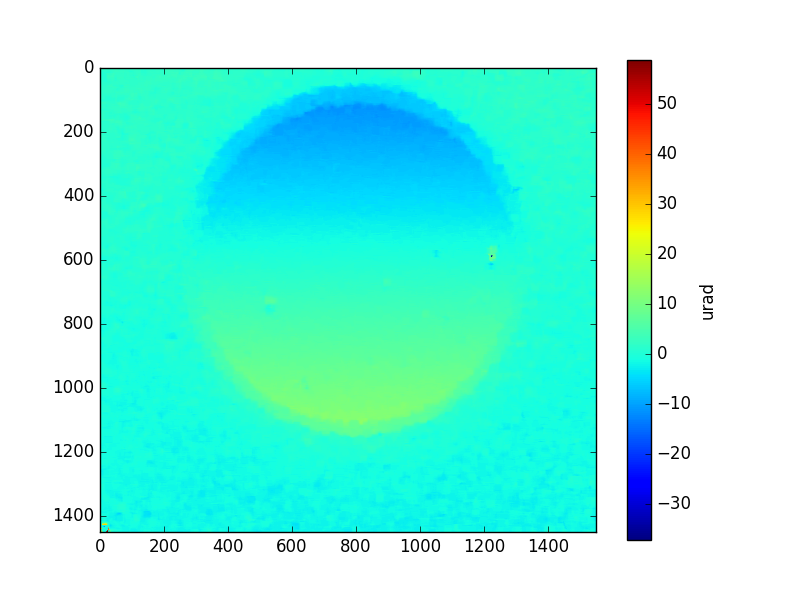
\includegraphics[width=0.4\linewidth]{img/SpeckDisV_E10001_edf_ref_start0001_1-10_edf}}};
	\only<5>{\draw[red, very thick] (-1.2, -3.7) rectangle (2.9, 3.7)};
	\only<5>{\draw[white] (-1, 0.2) rectangle node[black]{Horizontaler Gradient} (2.5, 0.5)};
	\only<5>{\draw[white] (-1, -3.6) rectangle node[black]{Vertikaler Gradient} (2.5, -3.1)};
	\only<5>{\draw[red, very thick] (-4.1, -0.7) -- (-1.2, 3.7)};
	\only<5>{\draw[red, very thick] (-4.1, -1.4) -- (-1.2, -3.7)};
	
	\only<6-7>{\draw[red, very thick] (-5.9, -2.5) rectangle (-4.1, -1.85)};
	\only<6>{\node at (-2,0) {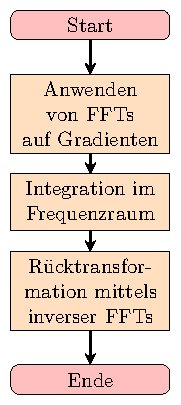
\includegraphics[width=0.17\linewidth]{tex/graph_fc}}};
	
	\only<6>{\draw[red, very thick] (-4.1, -1.85) -- (-3, 2.3)};
	\only<6>{\draw[red, very thick] (-4.1, -2.5) -- (-3, -2.3)};
	\only<6>{\draw[red, very thick] (-3, -2.3) rectangle (-0.9, 2.3)};
	
	\only<7>{\node at (1,0) {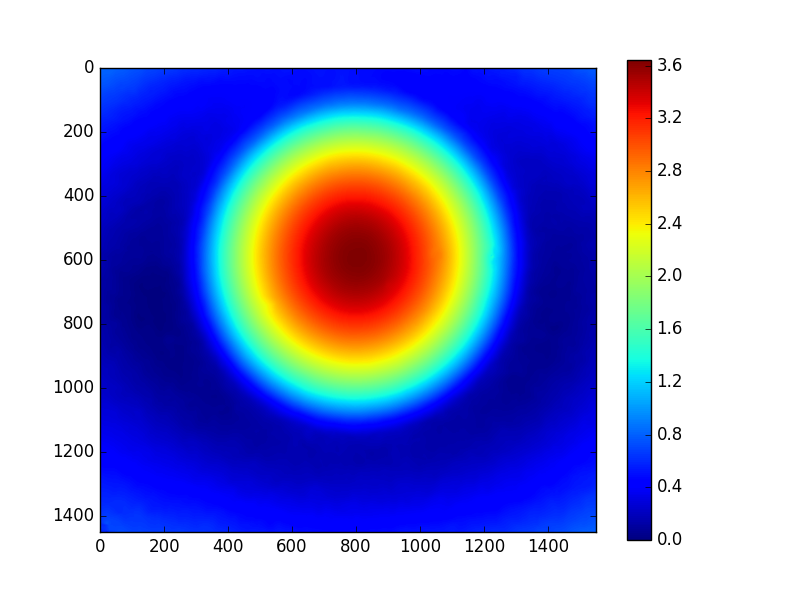
\includegraphics[width=0.6\linewidth]{img/2D_E10001_edf_ref_start0001_1-10_edf}}};
	\only<7>{\draw[red, very thick] (-2, -3) rectangle (3.6, 2.2)};
	\only<7>{\draw[white] (-1, -2.7) rectangle node[black]{Integrierte Gradientenmatrix} (2.5, -2.9)};
	\only<7>{\draw[red, very thick] (-4.1, -1.85) -- (-2, 2.2)};
	\only<7>{\draw[red, very thick] (-4.1, -2.5) -- (-2, -3)};
	\end{tikzpicture}
}
	\only<6-7> {\scalebox{0.9}{
			\begin{tikzpicture}
			\node at (-5,0) {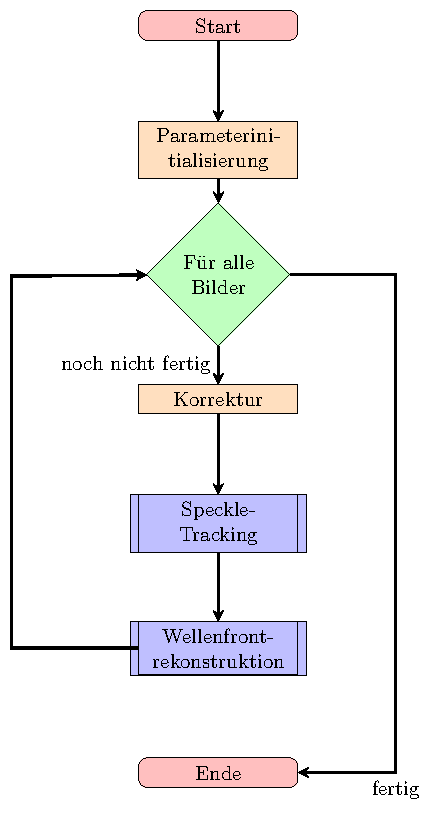
\includegraphics[width=0.35\linewidth]{tex/graph_main}};
			\only<2-4>{\node at (-2,0) {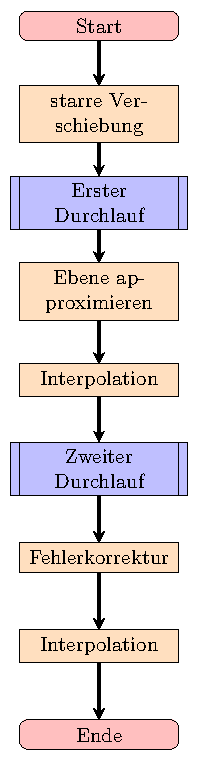
\includegraphics[width=0.17\linewidth]{tex/graph_speckle}}};
			
			\only<2>{\draw[red, very thick] (-5.9, -1.4) rectangle (-4.1, -0.7)};
			\only<2>{\draw[red, very thick] (-4.1, -0.7) -- (-3, 3.7)};
			\only<2>{\draw[red, very thick] (-4.1, -1.4) -- (-3, -3.7)};
			\only<2>{\draw[red, very thick] (-3, -3.7) rectangle (-0.9, 3.7)};
			
			
			\only<3-4>{\draw[red!25, very thick] (-5.9, -1.4) rectangle (-4.1, -0.7)};
			\only<3-4>{\draw[red!25, very thick] (-4.1, -0.7) -- (-3, 3.7)};
			\only<3-4>{\draw[red!25, very thick] (-4.1, -1.4) -- (-3, -3.7)};
			\only<3-4>{\draw[red!25, very thick] (-3, -3.7) rectangle (-0.9, 3.7)};
			
			\only<3>{\draw[red, very thick] (-2.95, 1.4) rectangle (-1.05, 2.07)};
			
			\only<4>{\draw[red, very thick] (-2.95, -1.2) rectangle (-1.05, -0.55)};
			
			\only<5>{\draw[red, very thick] (-5.9, -1.4) rectangle (-4.1, -0.7)};
			\only<5>{\node at (1,2.1) {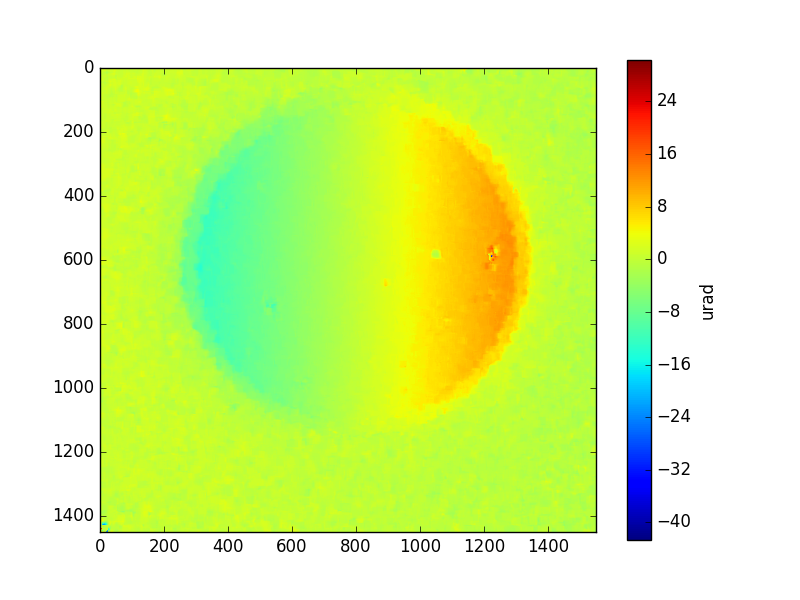
\includegraphics[width=0.4\linewidth]{img/SpeckDisH_E10001_edf_ref_start0001_1-10_edf}}};
			\only<5>{\node at (1,-1.6) {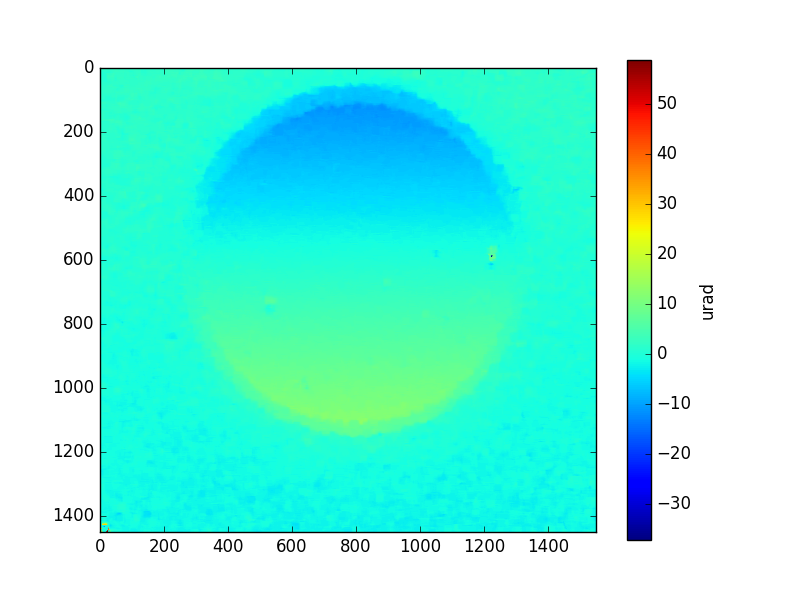
\includegraphics[width=0.4\linewidth]{img/SpeckDisV_E10001_edf_ref_start0001_1-10_edf}}};
			\only<5>{\draw[red, very thick] (-1.2, -3.7) rectangle (2.9, 3.7)};
			\only<5>{\draw[white] (-1, 0.2) rectangle node[black]{Horizontaler Gradient} (2.5, 0.5)};
			\only<5>{\draw[white] (-1, -3.6) rectangle node[black]{Vertikaler Gradient} (2.5, -3.1)};
			\only<5>{\draw[red, very thick] (-4.1, -0.7) -- (-1.2, 3.7)};
			\only<5>{\draw[red, very thick] (-4.1, -1.4) -- (-1.2, -3.7)};
			
			\only<6-7>{\draw[red, very thick] (-5.9, -2.5) rectangle (-4.1, -1.85)};
			\only<6>{\node at (-2,0) {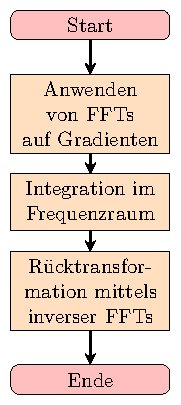
\includegraphics[width=0.17\linewidth]{tex/graph_fc}}};
			
			\only<6>{\draw[red, very thick] (-4.1, -1.85) -- (-3, 2.3)};
			\only<6>{\draw[red, very thick] (-4.1, -2.5) -- (-3, -2.3)};
			\only<6>{\draw[red, very thick] (-3, -2.3) rectangle (-0.9, 2.3)};
			
			\only<7>{\node at (1,0) {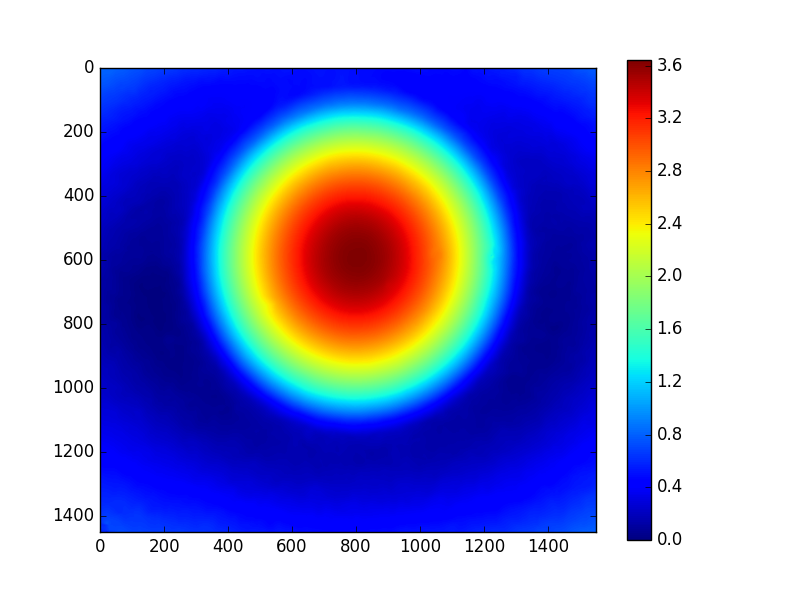
\includegraphics[width=0.6\linewidth]{img/2D_E10001_edf_ref_start0001_1-10_edf}}};
			\only<7>{\draw[red, very thick] (-2, -3) rectangle (3.6, 2.2)};
			\only<7>{\draw[white] (-1, -2.7) rectangle node[black]{Integrierte Gradientenmatrix} (2.5, -2.9)};
			\only<7>{\draw[red, very thick] (-4.1, -1.85) -- (-2, 2.2)};
			\only<7>{\draw[red, very thick] (-4.1, -2.5) -- (-2, -3)};
			\end{tikzpicture}
			\footnote{\citeall{fc88}}
	}}
\end{frame}

\begin{frame}{Initialisierung}
	\begin{center}
		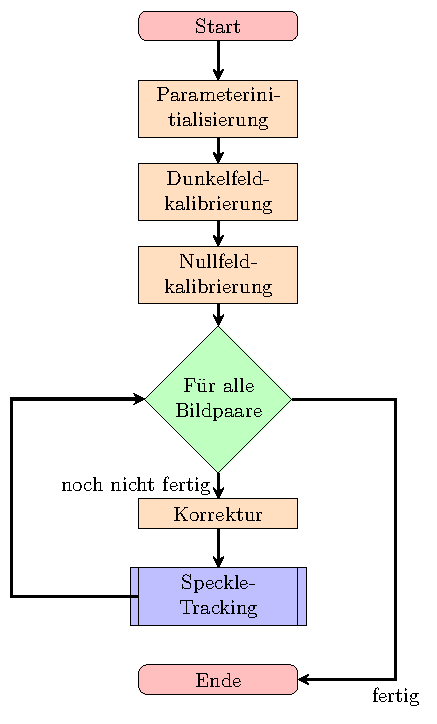
\includegraphics[width=0.4\linewidth]{tex/graph_init}
	\end{center}
\end{frame}

\iffalse

\subsection{Komplexität}
\begin{frame}[allowframebreaks]
\frametitle{Komplexität}
\begin{center}
	$ n $ -- Anzahl der Pixel; $ m $ -- Anzahl der Bilder \\
\end{center}
\textbf{Initialisierung:} \\
\setlength\extrarowheight{5pt}
\begin{center}
	\begin{tabular}{| >{\centering\arraybackslash}m{4cm} | >{\centering\arraybackslash}m{5cm} |}
		\hline
		Untergrund bestimmen & $ \mathcal{O}(m * n) $ \\ \hline
		Nullfeld-Kalibrierung & $ \mathcal{O}(m * n) $ \\ \hline
		Streueffekterkennung & $ \mathcal{O}(m^2 * \frac{n * corrSize * log(corrSize)}{(underSample * gridResol)^2}) \approx \mathcal{O}(m^2 * n^2 * log(n)) $ \\ \hline
	\end{tabular}
\end{center}
\vspace{.5cm}
\textbf{$ \Rightarrow $ Gesamtkomplexität:} $ \approx \mathcal{O}(m^2 * n^2 * log(n)) $

\framebreak

\begin{center}
	$ n $ -- Anzahl der Pixel; $ m $ -- Anzahl der Bilder \\
\end{center}
\textbf{Hauptroutine:} \\
\setlength\extrarowheight{5pt}
\begin{center}
	\begin{tabular}{| >{\centering\arraybackslash}m{4cm} | >{\centering\arraybackslash}m{5cm} |}
		\hline
		Bild-Präprozessierschritte & $ \mathcal{O}(m * n) $ \\ \hline
		Speckle-Tracking & $ \mathcal{O}(m * \frac{n * corrSize * log(corrSize)}{(underSample * gridResol)^2}) \approx \mathcal{O}(m * n^2 * log(n))$ \\ \hline
		Rekonstruktion der Wellenfront & $ \mathcal{O}(m * n * log(n)) $ \\ \hline
	\end{tabular}
\end{center}
\vspace{.5cm}
\textbf{$ \Rightarrow $ Gesamtkomplexität:} $ \approx \mathcal{O}(m * n^2 * log(n)) $
\end{frame}

\fi
\section{Performance-Analyse des derzeit fast durchgängig seriellen Codes}

\subsection{Datensets}
\begin{frame}{Datensets}
	\textbf{Initialisierung:}
	\begin{itemize}
		\item<2-> Detector Distortion
		\begin{itemize}
			\item ROI Größe: 1848x1848
			\item Gitterauflösung: 4
			\item Korrelationsgröße: 41
		\end{itemize}
	\end{itemize}
	\textbf{Hauptroutine:}
	\begin{itemize}
		\item<3-> Experiment 6
		\begin{itemize}
			\item ROI Größe: 1450x1450 (Bild), 550x550 (Template)
			\item Gitterauflösung: 1
			\item Korrelationsgröße: 91
			\item unterschiedliche Pixelgröße
		\end{itemize}
		\item<4-> Lenses
		\begin{itemize}
			\item ROI Größe: 1450x1550 (Bild), 1450x1550 (Template)
			\item Gitterauflösung: 1
			\item Korrelationsgröße: 41
			\item gleiche Pixelgröße
		\end{itemize}
	\end{itemize}
\end{frame}

\subsection{Gesamtlaufzeit}
\begin{frame}[allowframebreaks]
\frametitle{Gesamtlaufzeit}
	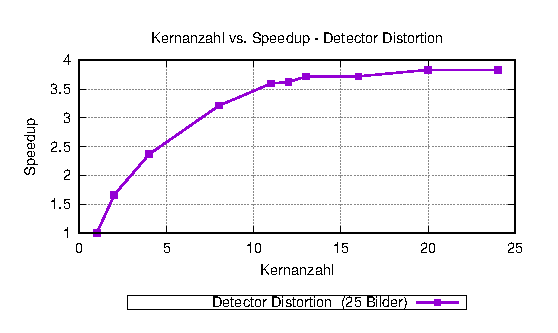
\includegraphics[width=0.9\linewidth]{img/times_detector_distortion}
	\begin{center}
		\scriptsize
		Python 2.7, 2x Intel(R) Xeon(R) E5-2680 v3 (12 Kerne) @ 2.50GHz, kein MultiThreading
	\end{center}
\framebreak
	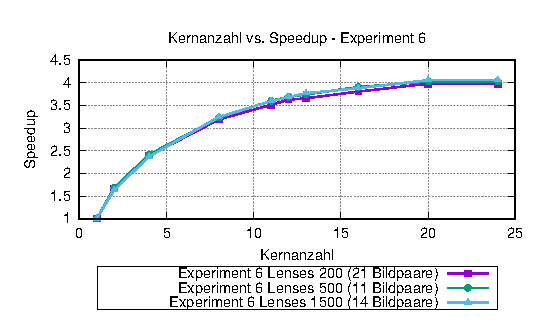
\includegraphics[width=0.9\linewidth]{img/times_exp6}
	\begin{center}
		\scriptsize
		Python 2.7, 2x Intel(R) Xeon(R) E5-2680 v3 (12 Kerne) @ 2.50GHz, kein MultiThreading
	\end{center}
\framebreak
	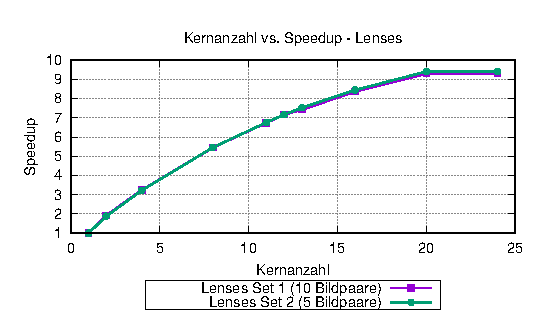
\includegraphics[width=0.9\linewidth]{img/times_lenses}
	\begin{center}
		\scriptsize
		Python 2.7, 2x Intel(R) Xeon(R) E5-2680 v3 (12 Kerne) @ 2.50GHz, kein MultiThreading
	\end{center}
\framebreak
\end{frame}

\subsection{Profiling}
\begin{frame}[allowframebreaks]
\frametitle{Profiling}
	\begin{center}
		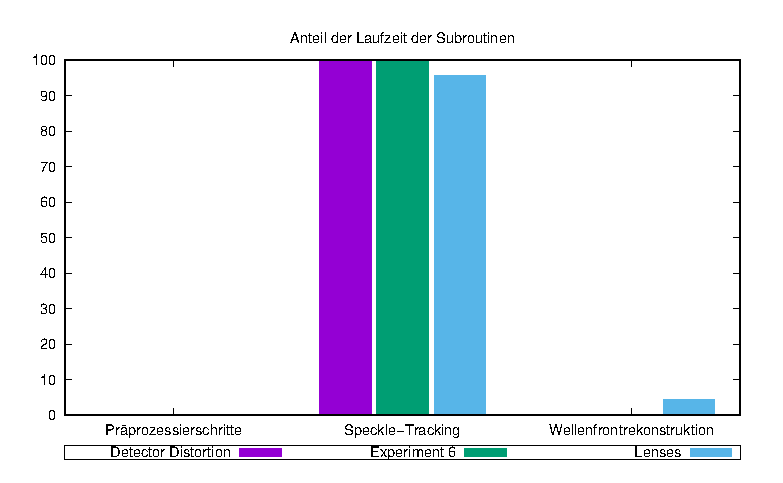
\includegraphics[width=0.74\linewidth]{img/main.eps}
		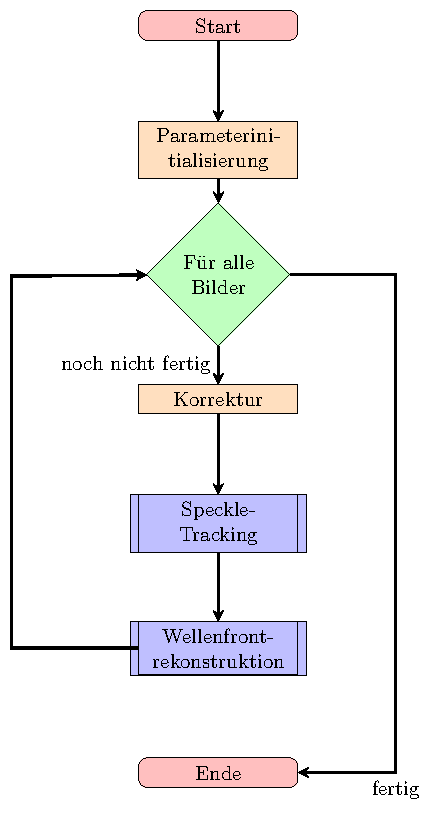
\includegraphics[width=0.25\linewidth]{tex/graph_main}
\framebreak
		
		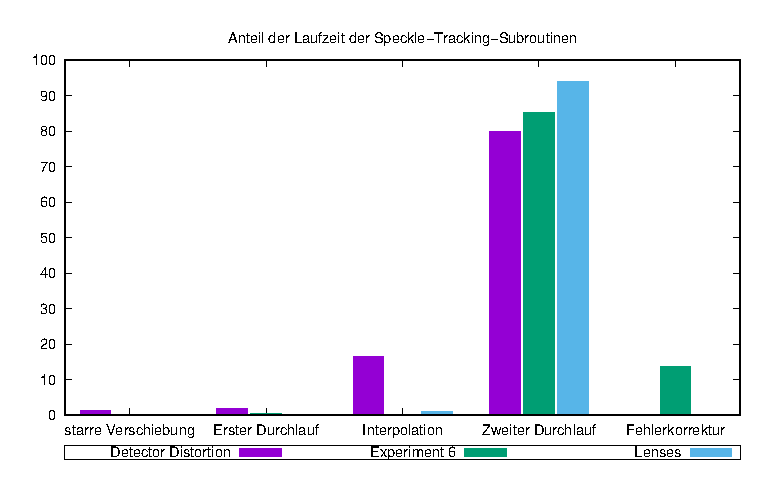
\includegraphics[width=0.84\linewidth]{img/speckle.eps}
		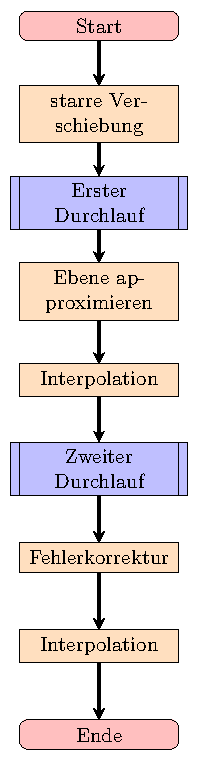
\includegraphics[width=0.15\linewidth]{tex/graph_speckle}
		
\framebreak
		
		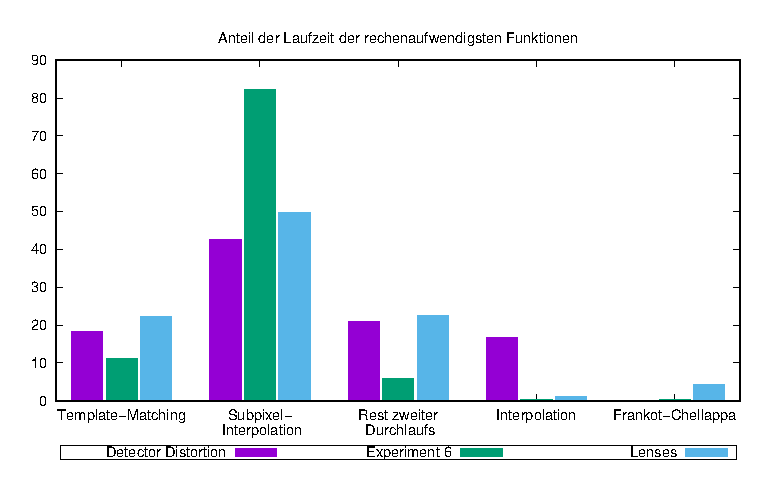
\includegraphics[width=0.94\linewidth]{img/slow.eps}\\
		\textbf{$ \Rightarrow $ über 95\%}
	\end{center}
\end{frame}
\section{Parallelisierung der kritischen Pfade für Vielkernarchitekturen}

\subsection{Möglichkeiten}
\begin{frame}{Möglichkeiten}
	\begin{itemize}
		\item Kompilieren
		\begin{uncoverenv}<2->
			\textbf{aber:} meist kein Speedup
		\end{uncoverenv}
		\item<3-> Parallelisierung
		\begin{uncoverenv}<4->
			\textbf{trivial möglich}
		\end{uncoverenv}
		\item<5-> Optimieren einzelner kritischer Pfade\\
		\begin{uncoverenv}<4->
			$\rightarrow$ C/C++ Portierung, optimierte Bibliotheken (numpy, numba, etc.), ...
		\end{uncoverenv}
	\end{itemize}
\end{frame}
\section{Stand der Arbeit}

\subsection{Jetziger Stand}
\begin{frame}{Jetziger Stand}
	\textbf{Bereits erledigt:}
	\begin{itemize}
		\item Evaluierung
		\item Performance-Analyse
		\item Kompilieren
	\end{itemize}
	
	\begin{uncoverenv}<2->
		\textbf{In Bearbeitung:}
		\begin{itemize}
			\item Parallelisieren
			\item Optimieren von reinem Python-Code
		\end{itemize}
	\end{uncoverenv}
\end{frame}

\subsection{Weiterer Plan}
\begin{frame}{Weiterer Plan}
\textbf{Noch geplant:}
\begin{itemize}
	\item Optimierung kritischer Pfade
	\begin{itemize}
		\item vermehrte Verwendung optimierter Bibliotheken
		\item C/C++ Portierung einzelner Funktionen
	\end{itemize}
	\item Validierung der parallelen Implementierung
	\item Performance-Messung der parallelen Implementierung
\end{itemize}
\end{frame}

\subsection{Probleme}
\begin{frame}{Probleme}
	\begin{itemize}
		\item Bugs in Referenzimplementierung
		\item<2-> Python Multithreading
		\begin{itemize}
			\item<3-> viele Profiler für Python, wenige mit Multithreading-Support
			\item<4-> Forken der kompletten Python-Umgebung nötig
		\end{itemize}
		\item<5-> schlechte Kompilierergebnisse
	\end{itemize}
\end{frame}
\appendix
\section<presentation>*{\appendixname}
\subsection<presentation>*{Weiterführende Literatur}

\begin{frame}[allowframebreaks]
  \frametitle<presentation>{Weiterführende Literatur}
    
 	{\footnotesize
 		
  	\printbibliography}
  
\end{frame}

\end{document}
